\chapter{Introduction}
\label{cha:Introduction}

\section{Motivation}
Firmware for industrial application requires intensive and thorough testing, that often happens in a behavioural manner. This denotes in testing from outside, via the systems interfaces. Quality measures, that inspect the inner processes of a firmware, allow additional insight to increase reliability and stability. Absence of such measures might lead to firmware containing major unnoticed errors. During execution of the firmware, these errors possibly cause malfunction and even destruction of the host system.

The project 'OCTane', a signal-generator, consists of firmware and hardware to control galvanometer-scanners. Galvanometer-scanners are key elements of OCT-systems. They allow the scanning of areas, instead of only point-wise measurements, by manipulating a laser-beam. Two separate steering-voltages enable this manipulation in x-, and y-direction. An existing microcontroller-board, providing two analogue outputs, hosts the firmware to generate such steering-voltages. USB-connectivity provides control over the unit. Additionally, the firmware must include a HAL (hardware abstraction layer), utilizing several miscellaneous functionalities of the microcontroller. This is an appropriate project to apply quality measures, to ensure adequate reliability of the resulting signal-generator. An insufficient level of quality might even lead to damage of attached components.

\section{Optical Coherence Tomography}
Optical coherence tomography (OCT) is an imaging method for the analysis of transparent and semi-transparent materials. It shows similarities to the measurement processes via ultrasound or radar. A light source applies an electromagnetic wave on the sample under test. Relevant properties of the resulting 'echoes' are their times of flight, as well as their intensities. This measured properties contain information of the sample-geometry, including the layer structure and also the maximum penetration depth of the applied wave. This creates a single point 1D-measurement, containing the lateral structure of the material. \\ 
A coherent broadband light source generates this electromagnetic wave in the visible, up to the near infrared spectrum. Coherent means, that several wave-bundles of a light source must have a fixed phase relationship to each other. This is necessary to obtain stable interference patterns. \\ 
For the detection of the echoes, conventional photodetectors or cameras do not suffice. On the one hand due to the propagation speed of light, on the other hand due to the low reflected light intensities. Therefore, OCT-systems use interferometry to detect the back reflected light. Fig ~\ref{OCTPrinciplesTDOCT} visualizes the structure of an interferometer, suitable for OCT-imaging. In interferometry, a laser beam is split into two waves. One wave travels on an optical reference path of known length, the other to the surface of the sample. The interferometer superimposes the reflections, the returning waves. Depending on the nature of the sample material, this results in constructive or destructive interference. A spectrometer detects these interferences and assembles several of them into an interferogram. \TODO{Bild-Quelle richtig verweisen} \\ 
\bildGr{h!}{OCT_Principles_TD_OCT.JPG}{Principle of time-domain OCT.}{OCTPrinciplesTDOCT}{0.9\textwidth}
The term 'A-scan' denotes a single point measurement and its depth information about the material under test. An aggregation of A-scans along a line (x-direction) across the sample material, forms a B-scan. Aggregation of B-scans along a line in the y-direction result in a volume scan, i.e. a spatial, three-dimensional image of the sample material. Relevant parameters of OCT systems are the penetration depth, the axial and lateral measurement range, axial and lateral resolution and the measurement speed. While the penetration depth of ultrasound typically reaches a few centimetres and a resolution in the millimetre range, OCT allows only to look a few millimetres below the surface, but with micrometer resolutions. Measurable areas, or field-of-view, in ultrasound is in the order of centimetres, with OCT in the order of millimetres. Achievable measurement speed results in up to 100kHz of A-scan rate. \\ 
The term 'optical coherence tomography' results on the one hand from the coherent light source. The other two parts of the name, 'tomos' means slice or section, and 'graphein' stand for writing or drawing, and both come from Greek. They reflect that the resulting image is an assembly of individual slices or sectional images. \\
Rotatably mounted mirrors, one for the x- one for the y- direction, allow for the manipulation of the light beam along the mentioned lines. The faster this rotation is possible, the higher the measurement speed of OCT-images. One widespread technical realization, allowing very fast rotation of the mirrors, is a galvanometer-mirror or -scanner.


\section{Galvanometer-Scanners}
Galvanometer scanners (colloquial: galvos) are highly dynamic opto-mechanical components, based on the classic galvanometer according to Hans Christian Oersted: A current-carrying conductor in the proximity of a rotatable, magnetizable object, e.g. a magnetic needle, deflects this object from its initial position. Wiring a high number of windings of the electric conductor around the deflectable object, creating an electrical inductance, a coil. This improves the low sensitivity of the described effect. Placing the coil between a rigidly positioned iron-cylinder inside and a permanent-magnet outside the coil, linearizes the relation between current and deflection angle to a first-order approximation.
\cite{keithleyHistory}. 
If this classic galvanometer carries a mirror as a rotatable object, it can manipulate optical paths, specifically: the beam-path of a point light source, in one space dimension. Feasible for technical applications is, that this manipulation happens nearly linear with the current at the galvo coil. The galvanometer-scanner in use for this master-thesis, already includes power-electronics for the conversion of control signals to the required coil-currents. Therefore, furthermore, only 'control signals' will be discussed, instead of currents and voltages. A combination of two galvanometer scanners in a suitable geometric arrangement, irradiated with a point laser, allows to manipulate this point in two dimensions. Such an arrangement is shown in fig. ~\ref{DetailGalvoOn}. At sufficient speed, at which the laser point is deflected, 2-dimensional contours illuminate the target area, resulting in a 'stationary' image for the human eye. It shall be noted, that only closed geometric figures are possible, as long as the light source itself cannot be turned off. These components are commercially available as laser scanner and used for light effects at music events, art installations and in discotheques. In OCT-systems, on the other hand, galvanometer scanners expand the measurement area from a single point of interest to an area. Scanning mentioned coherent light over an area of the examined sample, allows for three dimensional analysis of the sample. Steering  dedicated x- and a y-mirrors with a slow and a fast ramp, respectively, results in a rectangular illumination of the sample. This is the preferred illumination pattern for OCT-systems, as it allows raster scanning of samples.

\begin{figure}[h!]	\centering	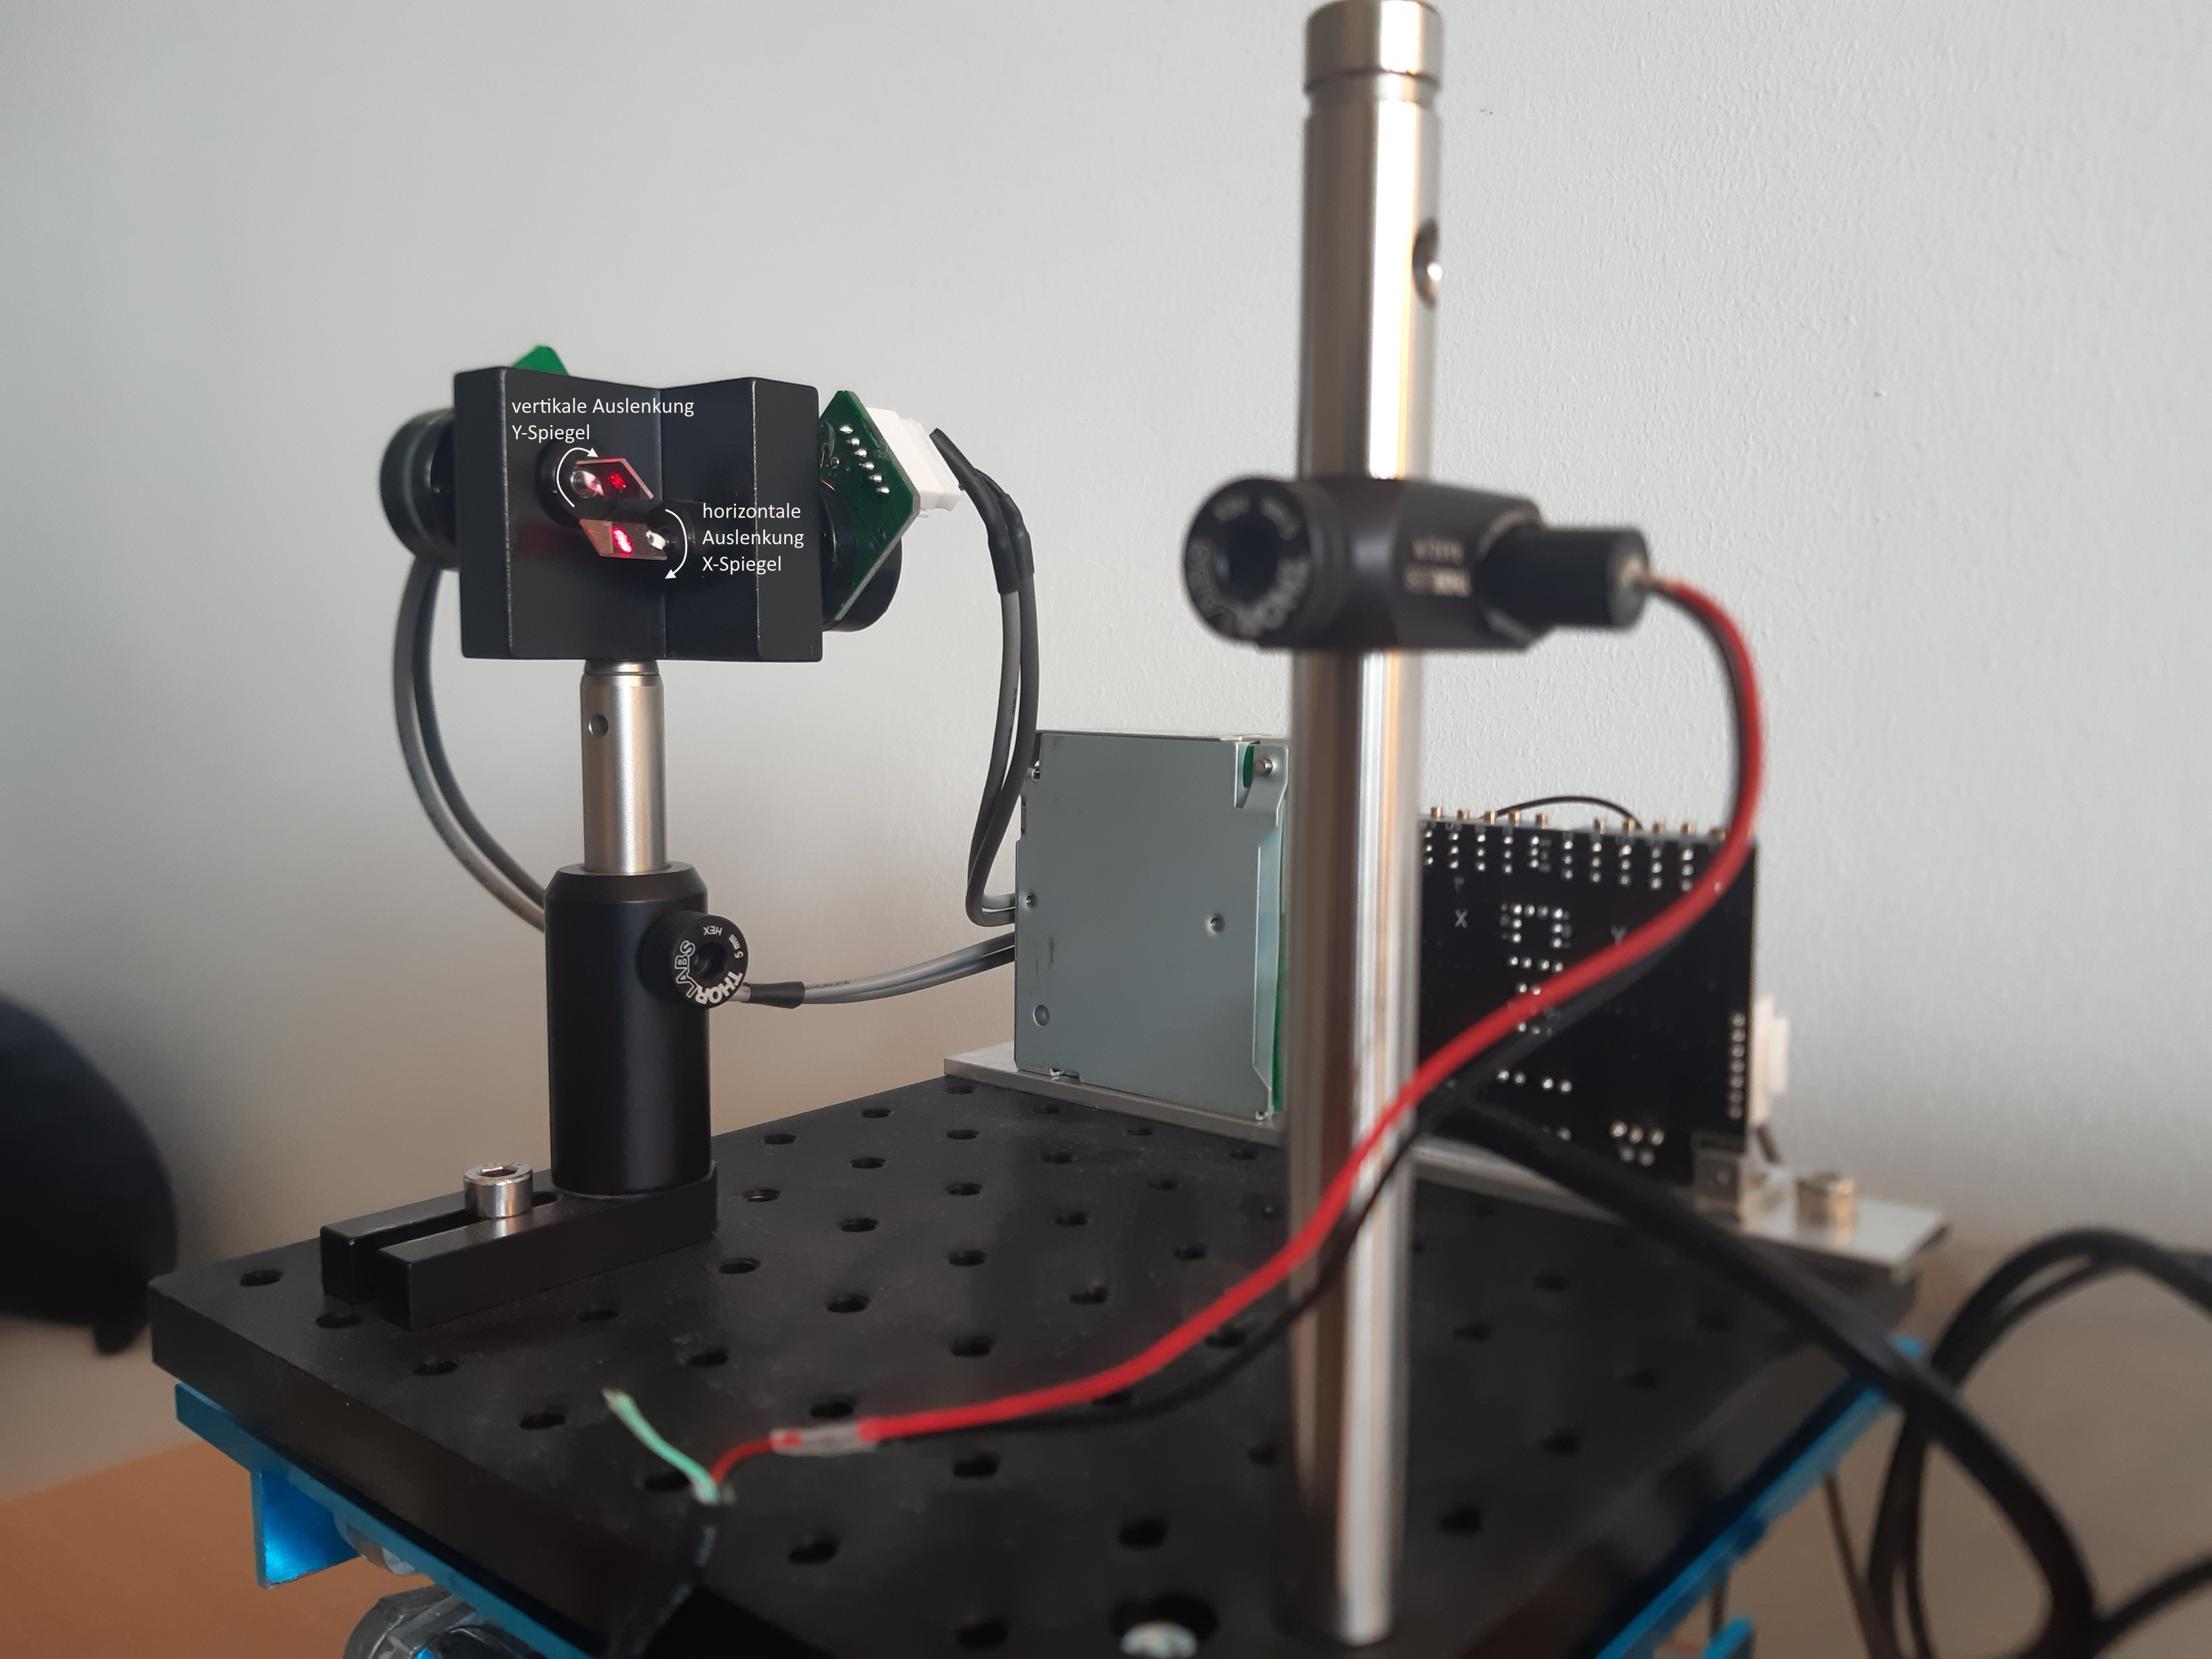
\includegraphics[width=\textwidth]{images/DetailGalvoOn.jpg}	\caption{experimental galvanometer-setup}	\label{DetailGalvoOn}	\end{figure}
% \begin{figure}[h!]	\centering	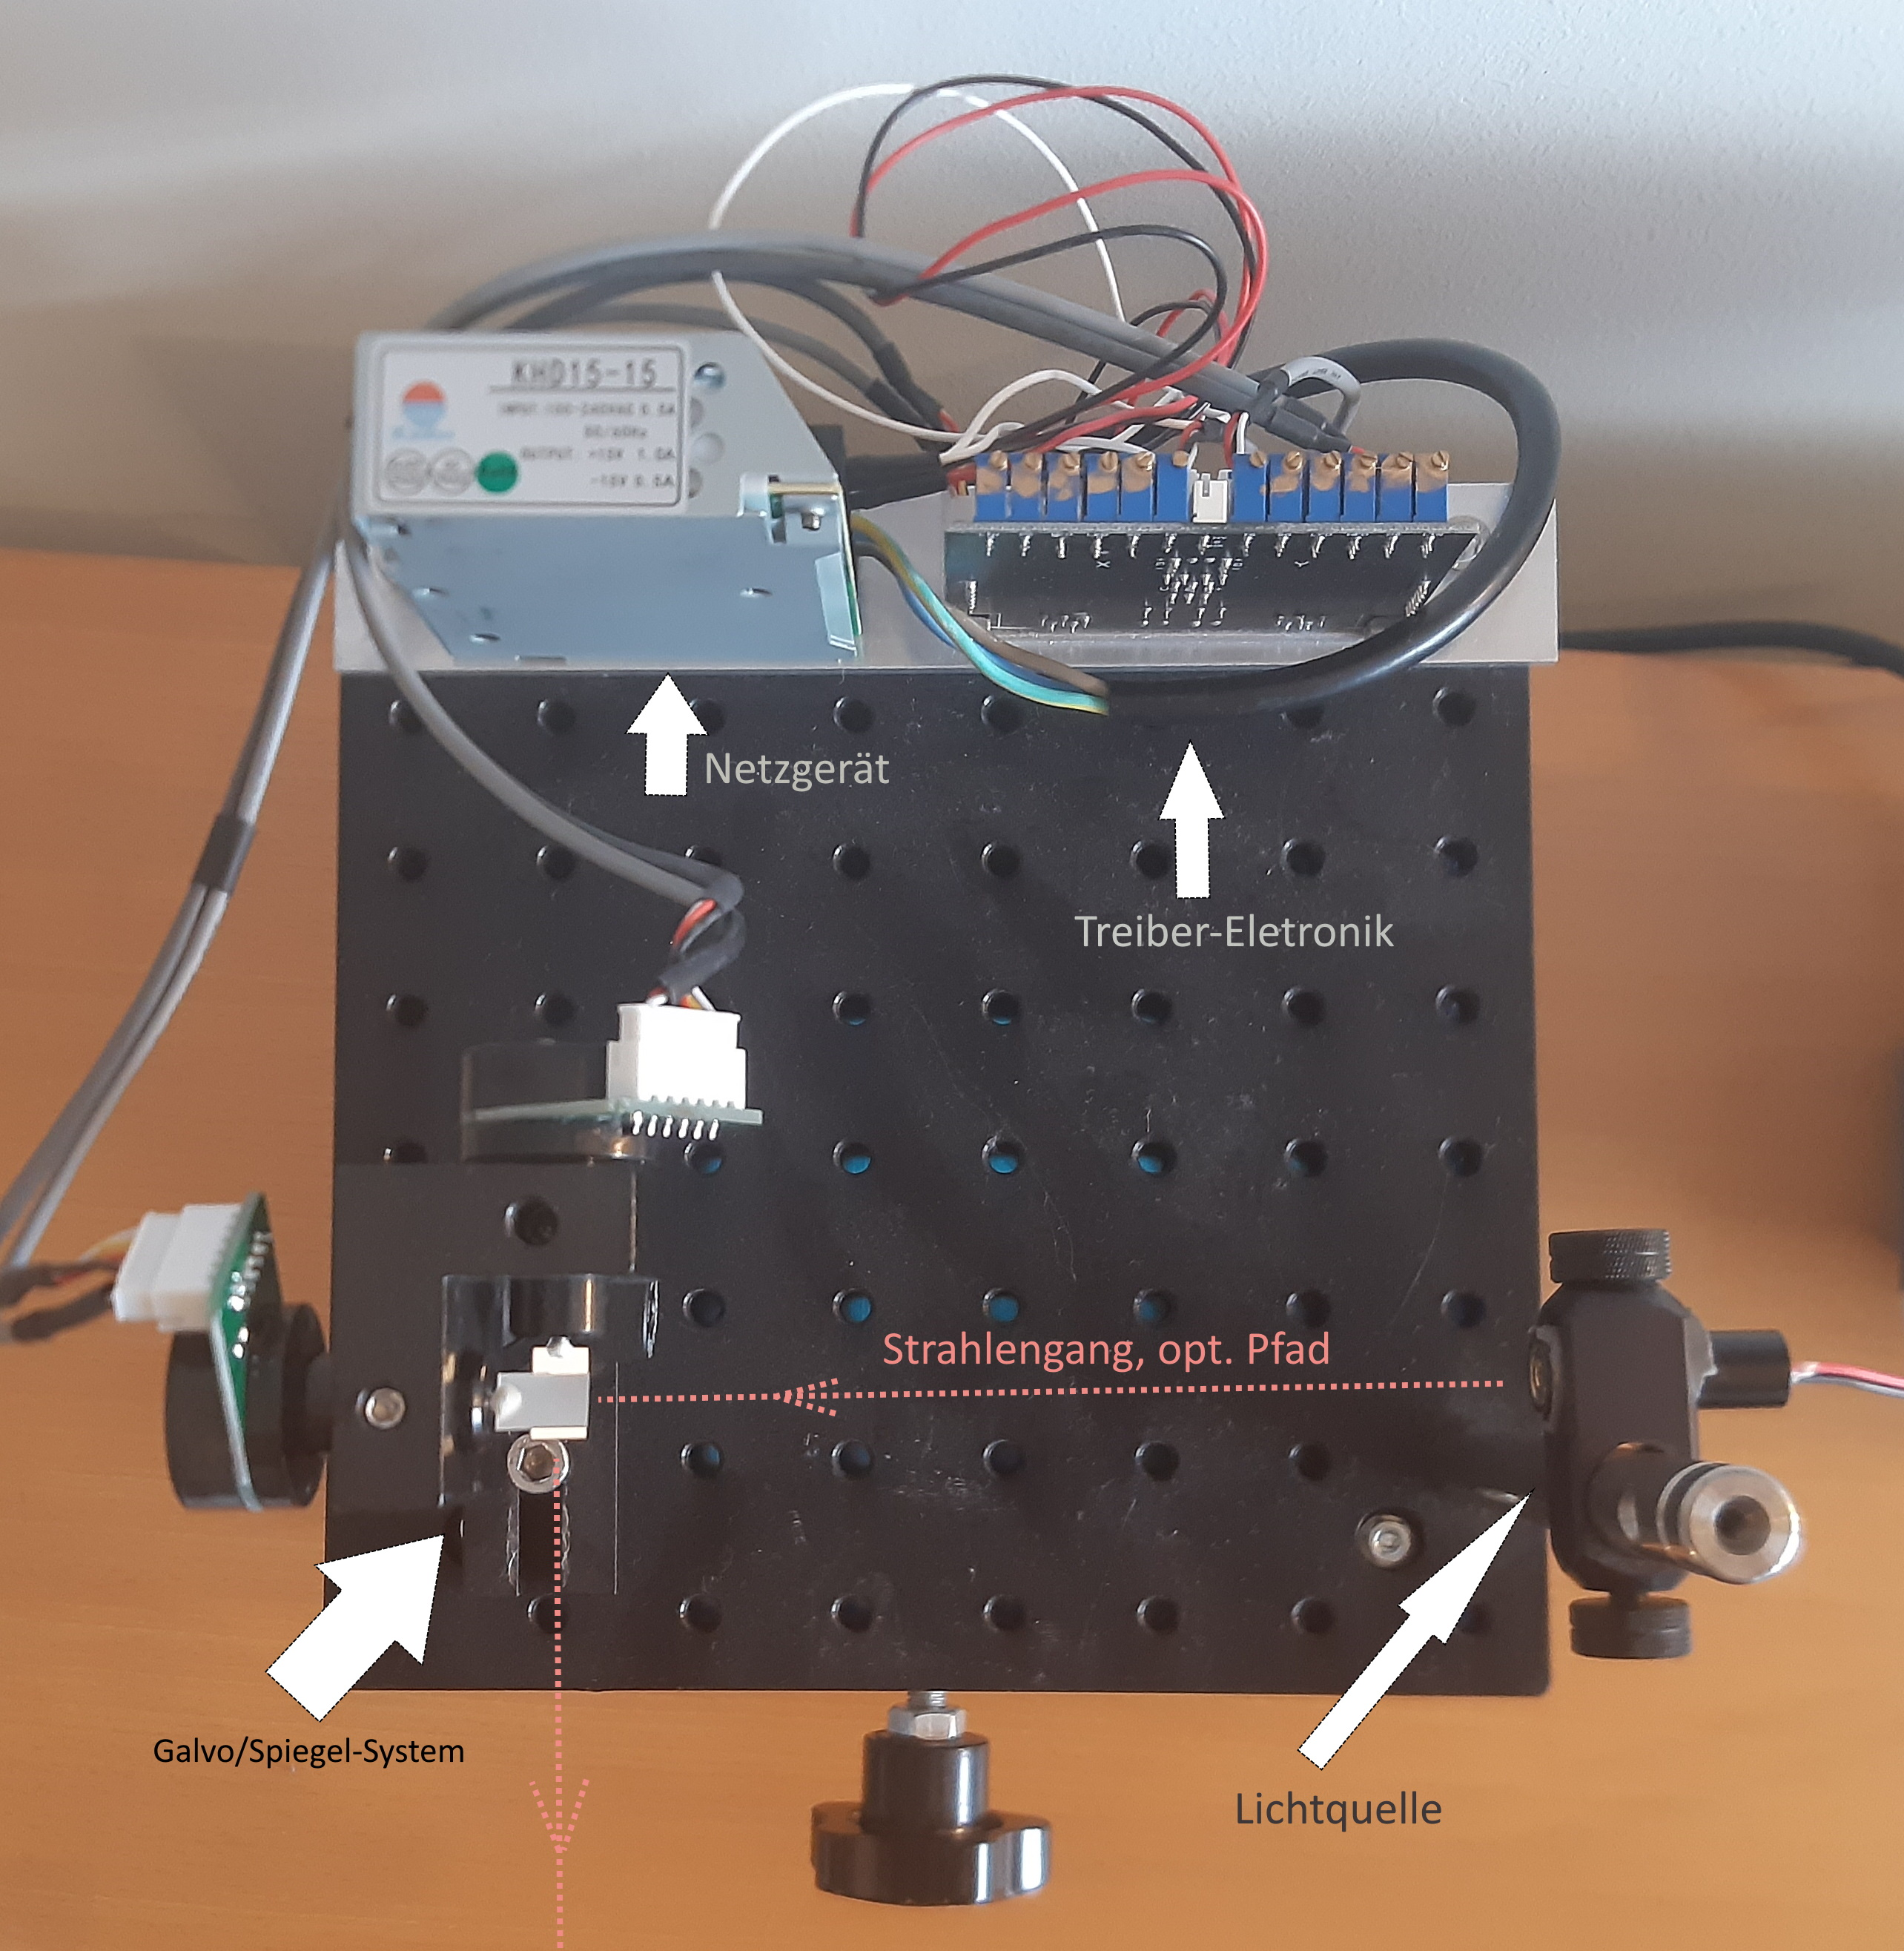
\includegraphics[width=\textwidth]{images/DutTop02.jpg}	\caption{Experimental setup, top-view.}	\label{DutTop02}	\end{figure}

\section{Control of Galvanometer-Scanners}
\begin{figure}[h!]	\centering	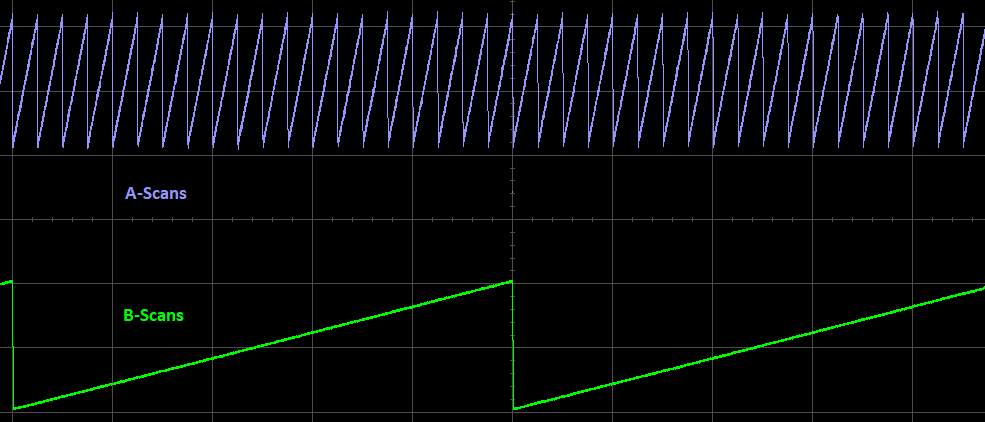
\includegraphics[width=\textwidth]{images/GalvoRamps01.png}	\caption{suitable signals for a rectangular scan.}	\label{GalvoRamps01}	\end{figure}
Commercially available galvanometer scanners usually allow control in the form of analogue voltage inputs with a range of $\pm$ 10volts. The angle of the rotated mirror follows that control-voltage in a linear manner for sufficiently low frequencies. Fig.~\ref{GalvoRamps01} shows suitable signal-forms to generate the rectangular scan-patterns, as described in the previous section. An existing microcontroller-board, including 16-bit analogue outputs, USB-connectivity and coaxial trigger outputs hosts a firmware. This firmware utilises the features of the underlying hardware to form an arbitrary signal generator for mentioned ramp-signals. Aside from signal-generation and USB-connectivity, the firmware has to provide access to additional features, such as user-controllable relays, utilisation of watchdog-timer, UART-, I2C- and SPI-ports as well as analogue inputs. The combination of hard- and firmware goes by the name OCTane. Fig. ~\ref{blocktane} demonstrates the integration of an OCTane into an OCT-system. \\ 
Quality measures have to accompany the implementation-process, to ensure sufficient reliability and stability. Obtaining the required performance data of a firmware for such quality measures constitutes a certain challenge. Analysis tools for software quality rely on a file-system to gather performance data. Implementing a file-system, though, is not feasible for the present firmware project, as it would only serve for measuring purposes and not contribute to the actual functionality. Analysing the firmware performance on the hosting system would exceed it's computational capabilities. An alternative way to transfer performance data from the host- to the analysing system is necessary. This leads to the scientific question: How to apply measures of software quality to a bare-metal firmware?
\bildGr{t!}{blocktane.pdf}{Integration of an OCTane}{blocktane}{\textwidth}
